\chapter{Methodology}\label{chapter:Methodology}
The following chapter explains how the first four steps of the plan are used in the forecasting task for this Interdisciplinary Project in detail. Step five, the results and evaluation, is discussed in the next chapters.\newline
First of all the specific problem will be defined properly. Next the information needed will be specified and gathered. This data is processed in the preliminary analysis and fitted to models.
\section{Problem Definition}\label{section:Problem Definition}
According to the process some general questions have to be solved before the forecast is started. For this purpose a stakeholder analysis is done and a SIPOC diagram is created (Tabular \ref{tab:sipoc}).

\begin{table}[]
\centering
\caption{SIPOC Diagram derived from the five basic steps}
\label{tab:sipoc}
\scalebox{0.75}{%
\begin{tabular}{|l|l|l|l|l|}
\hline
Supplier                                                                                                                                                                       & Input                                                                              & Process                                                                                                                    & Output                                                                 & Customer                                                                                       \\ \hline
\begin{tabular}[c]{@{}l@{}}Emanuel Pallua (COO)\\ Sebastian Sontheimer (BI)\\ Stefan Rothlehner(CTO)\\ Sergej Krauze (CTO)\\ Operations Team\end{tabular} & \begin{tabular}[c]{@{}l@{}}Knowledge\\ Experience\\ Historic Database\end{tabular} & \begin{tabular}[c]{@{}l@{}}Preliminary Analysis\\ Choosing Models\\ Fitting Models\\ Forecasting\\ Evaluating\end{tabular} & \begin{tabular}[c]{@{}l@{}}Forecast\\ Evaluation\\ Result\end{tabular} & \begin{tabular}[c]{@{}l@{}}Emanuel Pallua\\ Sebastian Sontheimer\\ Operation Team\end{tabular} \\ \hline
\end{tabular}}
\end{table}
Emanuel Pallua is identified as the first stakeholder. He is Chief of Operations at VOLO and the one who gave the forecast in order. Setting boundaries and demanding his needs makes him source and customer according to the SIPOC diagram. The goals of this forecast for him are to decrease idle times for drivers by being at the restaurant on time as well as increasing the freshness of the food by not leaving it ready at the restaurant for longer than necessary. In general he wants a robust forecasting process which can be continuously improved and automated in the future for daily usage. \newline
The second source and customer in one person is Sebastian Sontheimer who is with Business Intelligence. His aim is to optimize the whole process of VOLO, the same as for Emanuel Pallua. He supports the forecast process by adding his knowledge of the current numbers of VOLO. He suggests using only a few performance factors for the forecast, namely current slot (lunch, afternoon or dinner), current day, weekday, the week before and the weekday in the last month.\newline
On technical side there Stefan Rothlehner and Sergej Krauze, both Chief Technical Officers, as sources. Stefan Rothlehner is responsible for the backend and delivers the data. The information of the orders is extracted from the PostgreSQl database which is hosted on heroku. Sergej Krauze who is responsible for the Traveling Salesman Algorithm has the requirement that the language the forecast should be written in is Java. Since his work is already in Java it makes the whole integration a lot smoother.\newline
The last source and customer is the Operations Team since they are involved in the everyday business and will profit from the algorithm a lot. They support the algorithm with their real life scenario knowledge and require an operating forecast which is exact and needs no manual involvement.
\section{Gathering Information}\label{section:Gathering Information}
The information of the orders is taken from the database of the backend application which runs on heroku and is saved in PostgreSQL. The database is dumped at two dates in time. The data is downloaded into two sets, a training and a test set. The training set is to generate an initial forecast which is then validated with the test data set. This way relationships from the first forecast can be discovered and tested in the second one. The training data set was downloaded at the 26th of March 2015 to create a forecast which later can be compared to a test data set. This test data set was extracted from the server on the 29th of April. Speaking in number of orders, the csv file of the first extraction has 3034 entries while the second one has 4973 entries. The downloaded data sets were saved in comma separated values files, short csv files.\newline
This raw data has some weaknesses. The biggest one is the size of the gathered data. Forecasts need big amounts of information to generate a meaningful result. Since some restaurants have too few orders or a lot of bad data for the preparation times, additional expertise has to be put into the forecast. This information was taken from the operation teams. They have to deal with orders on a daily basis and right now have to "forecast" the point in time the driver has to be at the restaurant on their own. In their experience an estimation of around 15 minutes is a more or less accurate guess for most restaurants except for some which are known for their unpredictability.\newline
In order to use the datasets from the csv files, it has to be parsed into objects in the Java program. For this purpose a csv parser library is used. The library reads the csv file and matches the orders from the database to the OrderModel.class of the code. Not all attributes of the database are used, only the one related to the forecast are picked from the information. Since there is no tracking in the restaurant for the preparation time, it was decided to take the time interval from the point in time at which the restaurant knows from the order until the driver leaves the restaurant. In the process of volo, the printer in the restaurant prints the recipe at the same time the driver accepts the delivery, which is saved in the database as \texttt{accepted\_at}. The timestamp of the driver leaving the restaurant is saved in \texttt{delivery\_started\_at}. Since it is not the task to figure out the exact the preparation time but the time from when the order is send to the restaurant and when the driver can pick it up, no modification to the time are done.
\section{Preliminary Analysis}\label{section:Preliminary Analysis}
There are many factors which can influence the preparation times of the restaurant. Some are of external nature, some internal nature. The weather or season can have an effect on how busy the restaurant is which can cause different cooking times or when a cook is ill the restaurant can be overwhelmed by too many orders.\newline
Since only the timestamps of the status change are used, software failures have also be taken in account. There are also other factors, like marketing campaigns, which can influence the results, but this has not happened in the recorded time frame.\newline
In order to discover these patterns and get a feeling for the data the preliminary analysis is done.
\subsection{Raw Data Cleanup}\label{subsection:Raw Data Cleanup}
First of all the data has be cleaned and a rough overview for the dimensions of the data should be generated. This is done to get a feeling of the time frame a restaurant usually needs to prepare an order. This provides an estimation of what to expect and clue whether the result of a forecast is totally unrealistic or pretty close to what is possible. In addition to the average time analysis a visualization of the data is done as well. This is done in a time series plot on which it is very easy to see anomalies or patterns of the raw data.\newline

\begin{figure}[h]
\begin{center}
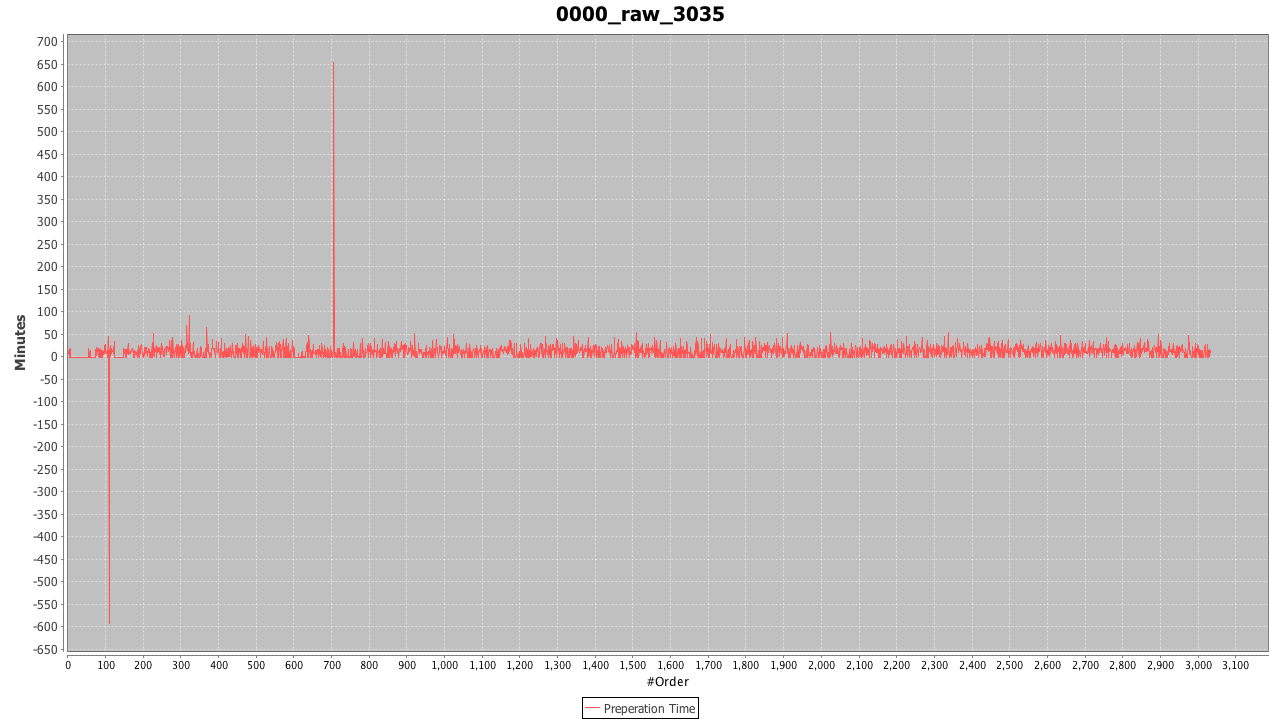
\includegraphics[width=10cm]{images/0000_raw_3035.png}
\caption{Observations of preparation time for each order without any data clean up}
\label{fig:0000_raw_3035}
\end{center}
\end{figure}

As the first step of the raw data cleanup, the training data is put into a time series graph (Fig. \ref{fig:0000_raw_3035}). This analysis reveals problems the data has. The training data set still contains unfinished orders, bugged order, which were finished at a wrong point of time, and orders which have corrupted timestamps. These three types of unusable orders receive a total time of "-1" since either their \texttt{accepted\_at} timestamp is missing or not readable. In case that the orders \texttt{delivery\_started\_at} timestamp is before the \texttt{accepted\_at} timestamp a negative value is visible. This events can be observed in many cases in the time series graph and result in an average preparation time of 12 minutes. In order to get good data these flaws have to be removed from the data set. This is done by ignoring all values which are below 0 minutes and increases the average preparation time to 16 minutes. This result is much higher than the first result but is free of wrong values which makes it more reliable. The data set is visualised in Figure \ref{fig:0000_invalid_2204}.

\begin{figure}[h]
\begin{center}
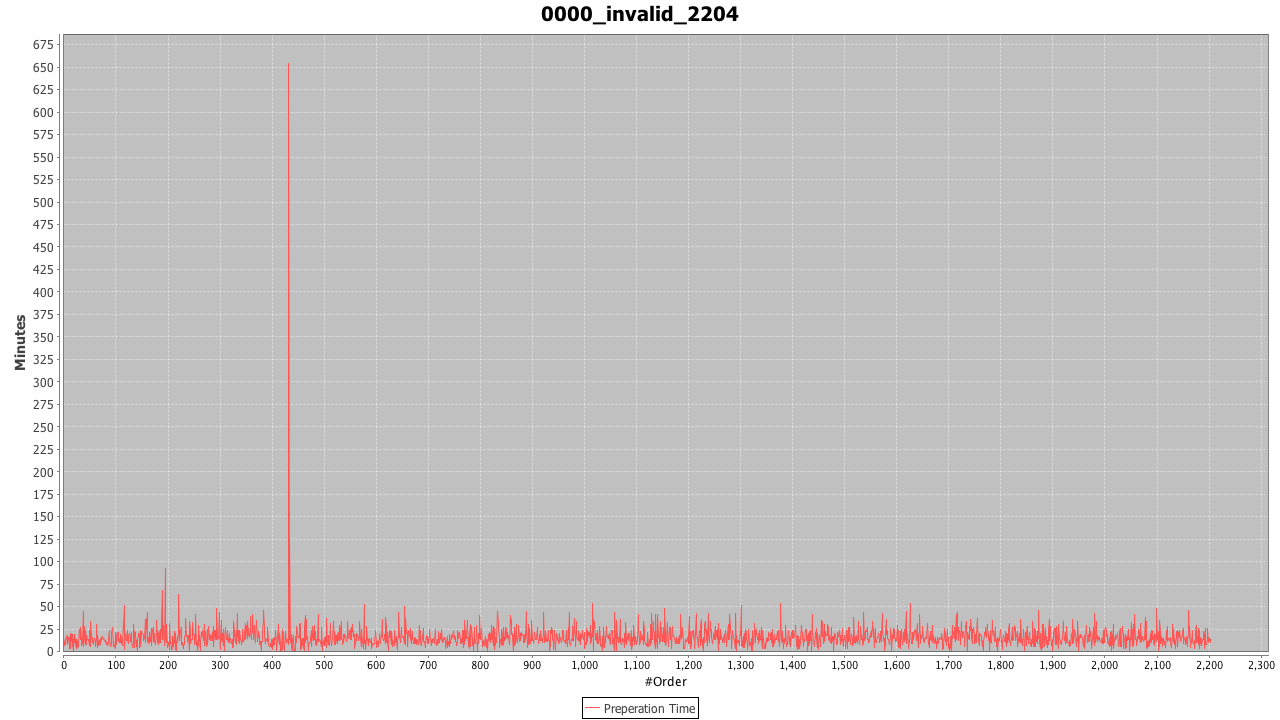
\includegraphics[width=10cm]{images/0000_invalid_2204.png}
\caption{Observations of preparation time for each order without invalid values}
\label{fig:0000_invalid_2204}
\end{center}
\end{figure}

After removing the obviously unusable orders the data looks a lot more usable. The only problem are the orders which were finished long after they have been started. It can be assumed that these times were either caused by bugged software or human error in the process and remove them from the data set. For this purpose the Grubbs training for outliers is applied to the dataset and all values seem not to come from a normally distributed population are removed. This results in an average preparation time of 15 minutes which is the same result as the operations team suggest to use as a basis. The visualisation of the data is done in Figure \ref{fig:0000_grubbed_2201}.

\begin{figure}[h]
\begin{center}
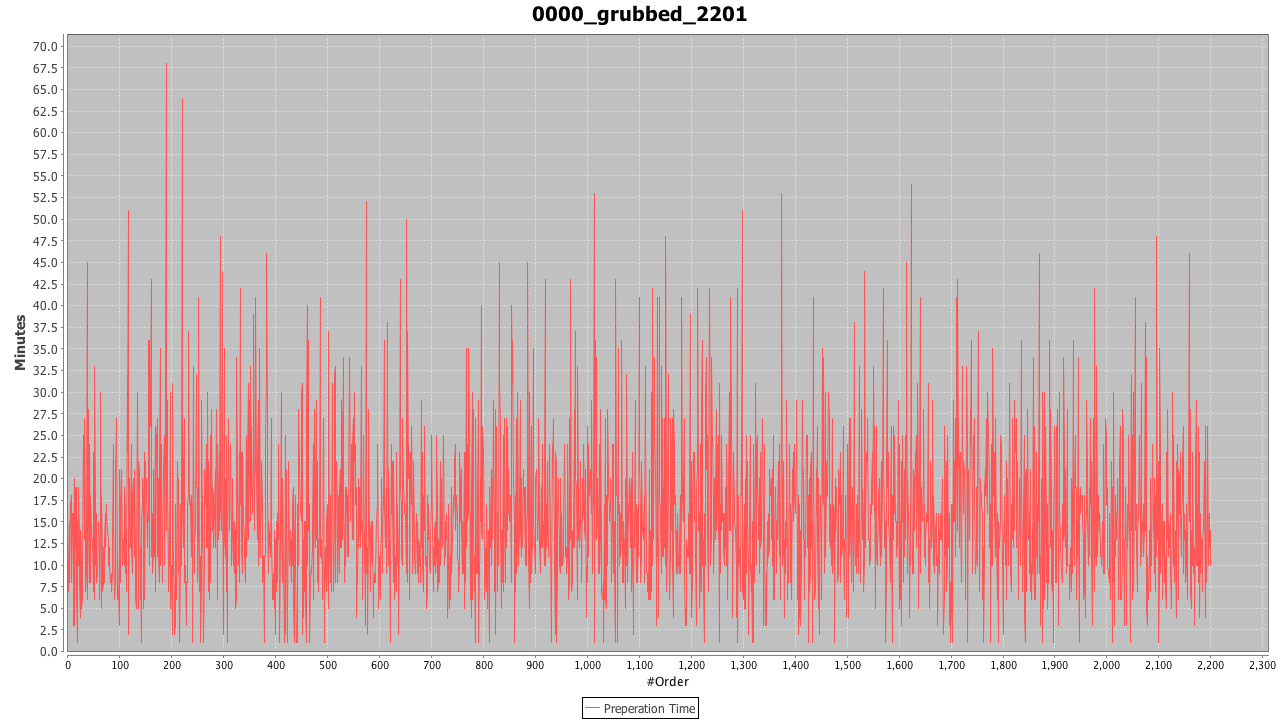
\includegraphics[width=10cm]{images/0000_grubbed_2201.png}
\caption{Observations of preparation time for each order without invalid values and outliers}
\label{fig:0000_grubbed_2201}
\end{center}
\end{figure}



Now the usable training dataset is extracted from the input data, it can be analyzed for patterns, trends or similarities. For this purpose a time component has to be introduced into the graph since putting order after order does not include it. That is why orders are summed up by day and visualized by average preparation time per day in Figure \ref{fig:0000_byDay_97}. The only usable information that can be extracted is that the average preparation time varies from day to day.

\begin{figure}[h]
\begin{center}
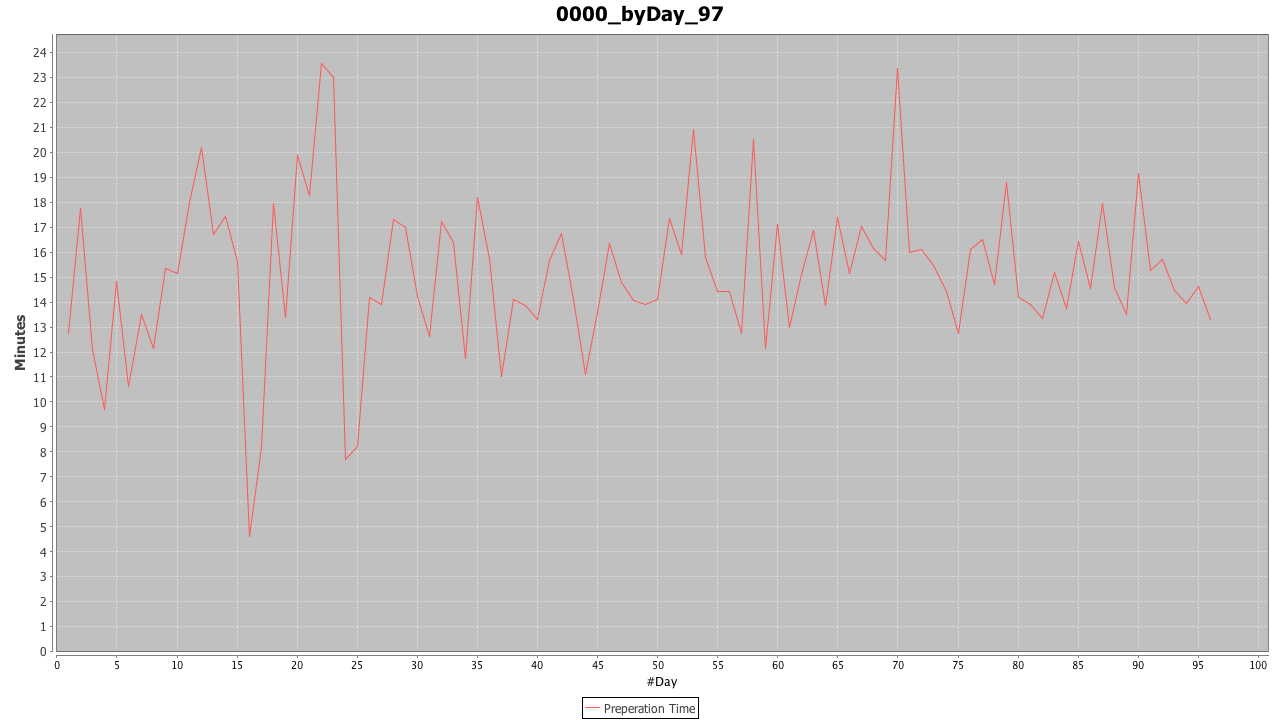
\includegraphics[width=10cm]{images/0000_byDay_97.png}
\caption{Average preparation time per day}
\label{fig:0000_byDay_97}
\end{center}
\end{figure}

Since no clear trend or pattern can be observed in a day by day analysis (Figure \ref{fig:0000_byDay_97}), a box and whisker diagram is created from the data (Figure \ref{fig:triple_boxWhisker}). It shows the median and average preparation time as line and point inside the box. The box represents the upper and lower quartile of preparation times in which 50 \% of the data is while the red whiskers visualize the area without outliers, which are red circles and a red triangle in case they are out of scale. The purpose of this graph is to give an overview of the set of values of the preparation time and the boundaries most of the orders are located in. The data was divided into different categories.\newline
The first diagram in Figure \ref{fig:triple_boxWhisker} on the left is on week basis. It was created to see if there is a trend over time as the company expertise grows. The only observation is that can be made is that after fluctuating preparation times in the first weeks it gets more constant towards the end.\newline
Since no conclusion can be drawn from this categorization, a box whisker diagram for each slot was created (Figure \ref{fig:triple_boxWhisker}, middle). The day is divided into three slots, the big meals, lunch and dinner, as well as the time between these, the afternoon, which should be not as busy as the meal times. The diagram shows no real difference in preparation times between the slots so this has to be inspected in a different categorization containing slots.\newline
This is done by visualizing the slots for each weekday in order to identify special behaviour since weekdays can have strong differences in terms of load for the restaurant (Figure \ref{fig:triple_boxWhisker}, right). This is done since it contains two different key information. Slots and weekdays alone do not have as much information as the two combined. For example on a sunday evening many people like to go to a restaurant and do not order while in the week offices sometimes order big deliveries for lunch. The values in the diagram do not vary that much which can be due to a low training dataset. It could also be separated between weekend and weekdays but there is not enough data to do this and gain additional information.\newline
The difference between slots on weekdays as well as between weekdays is more significant than all other diagrams before and should be considered when creating the model.

\begin{figure}[htp]

\centering
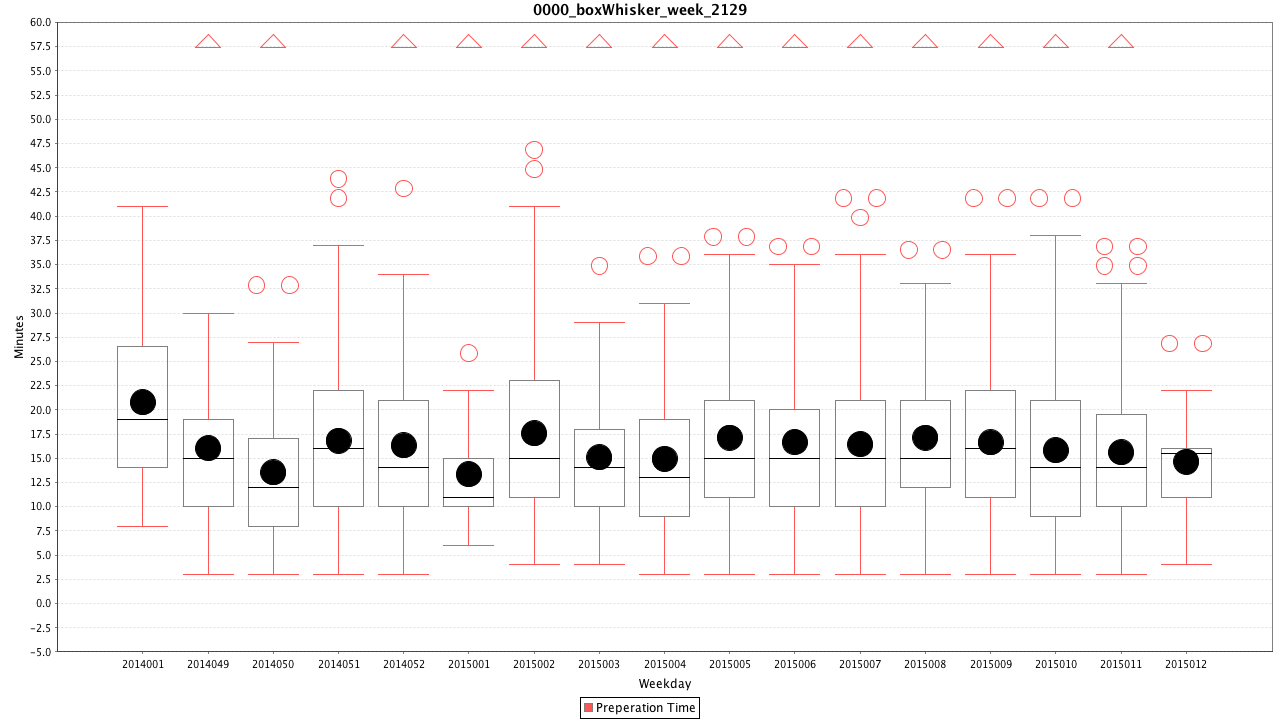
\includegraphics[width=.3\textwidth]{images/0000_boxWhisker_week_2129.png}\hfill
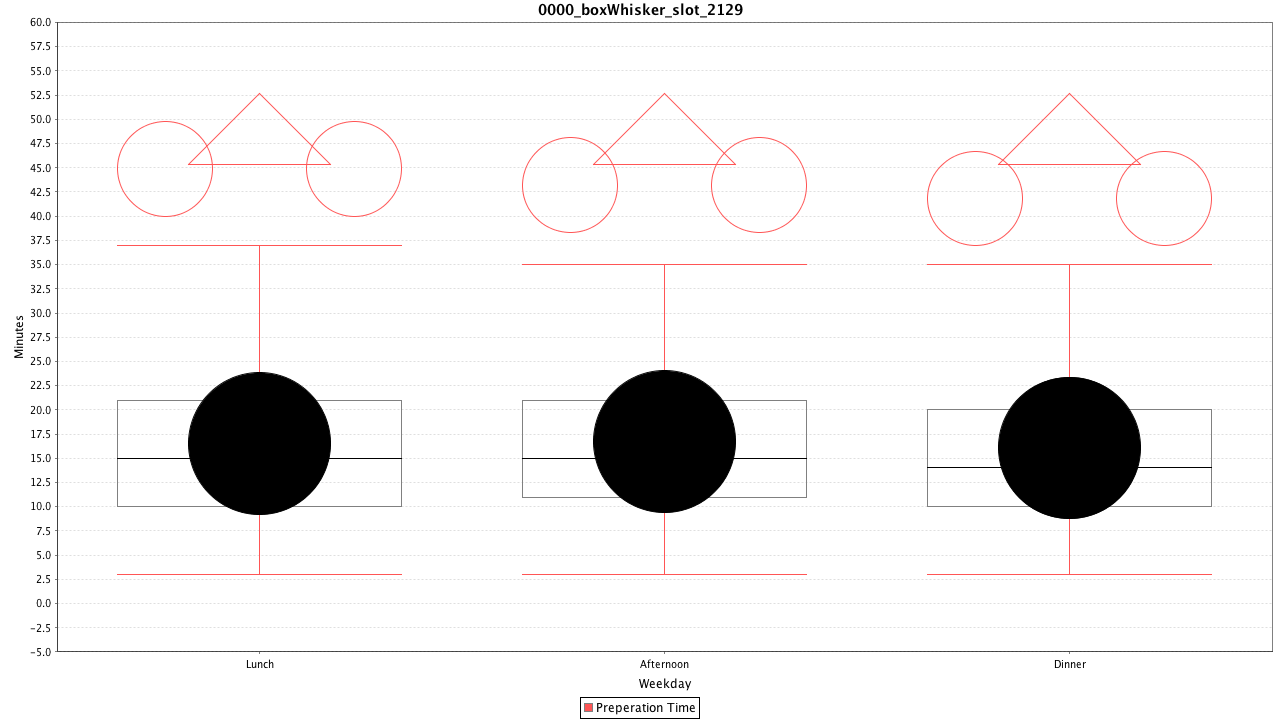
\includegraphics[width=.3\textwidth]{images/0000_boxWhisker_slot_2129.png}\hfill
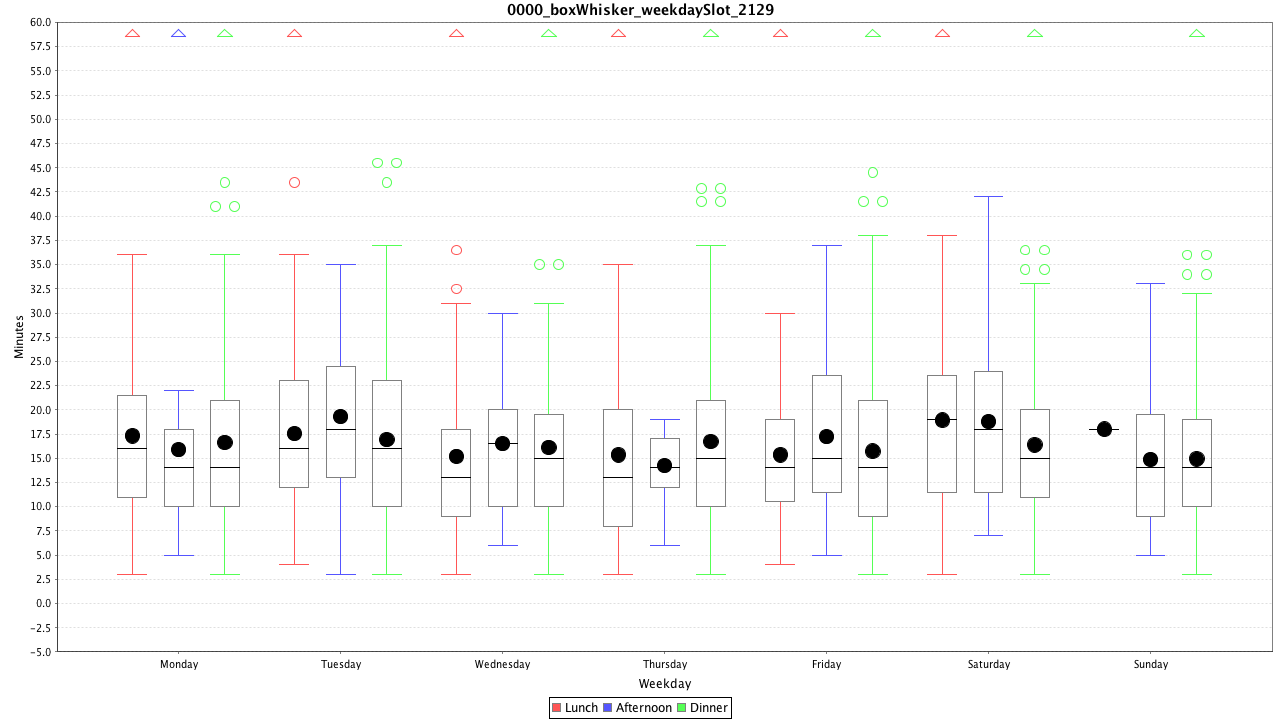
\includegraphics[width=.3\textwidth]{images/0000_boxWhisker_weekdaySlot_2129.png}

\caption{Different categorizations of the training data set}
\label{fig:triple_boxWhisker}

\end{figure}

All these lessons learned from the clean up of the data is also applied to the test data set which is used later.

\subsection{Restaurant Wise Proceeding}\label{subsection:Restaurant Wise Proceeding}
Before creating the model there should also be tested whether the restaurant has a significant impact on the preparation time.\newline
What was learned from the Operation Team is that restaurants are very different from each other. There are restaurants, which have already pre-cooked ingredients, others have a very simple way of preparing the meal, like sandwiches, and others are crowded at a certain time and will take longer. A pizzeria has other preparation times than a burrito take away.\newline
In order to get the best forecast possible for each restaurant they have to be looked at separately. For this purpose a popular restaurant should be chosen because it has the the largest amount of orders and is thus a good representation. Normally this is a bad idea since there is already a limited set of data but in this case the gains are more significant since the restaurants are so different and should be looked at individually.\newline
The restaurant with the most orders in the database is yum2take and is chosen. yum2take is a thai take-away and restaurant and the first restaurant volo delivered from. It is also close to the office which results in a bigger number of the driver being too early than being too late. Being early has the average that it does not falsifies our data as being late does. This is due to the timestamp \texttt{delivery\_started\_at} is being set as the driver leaves the restaurant. In order to get a first look at the data, a diagram categorized by slot for each weekday is created in Figure \ref{fig:1_boxWhisker_weekdaySlot_686}.
\begin{figure}[h]
\begin{center}
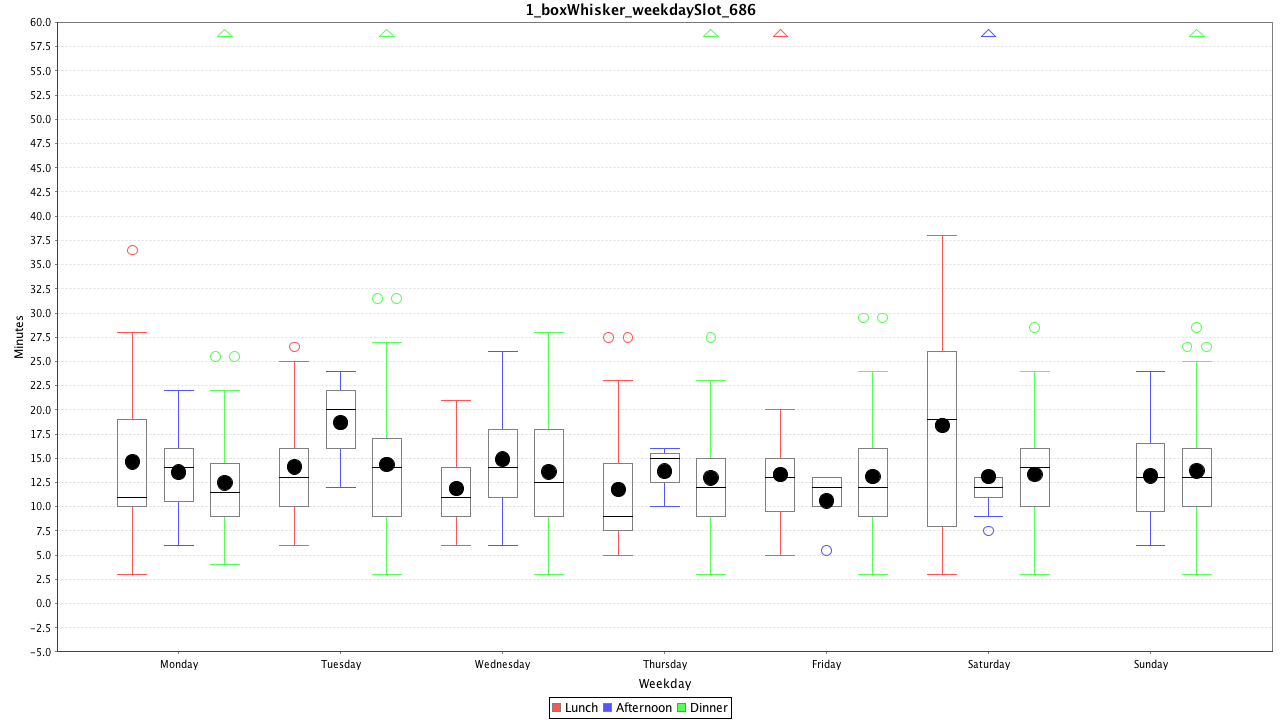
\includegraphics[width=10cm]{images/1_boxWhisker_weekdaySlot_686.png}
\caption{Observations of preparation time for orders at yum2take without invalid values and outliers}
\label{fig:1_boxWhisker_weekdaySlot_686}
\end{center}
\end{figure}
The distribution in the diagram for yum2take is clearly different from the overall visualization. This consolidates the assumption that restaurants should be looked at separately. The average times also have been different. For the raw data 10.2 minutes are the average, when cleaning the data from invalid values it increased to 13.5 minutes and without the outliers it lowered to 13.1 minutes.
\section{Choosing and Fitting Models}\label{Choosing and Fitting Models}
After the preliminary analysis it is time to fit the data to models for the forecast.
\subsection{Categorizing of Orders}\label{subsection:Categorizing by Order}
With these different first insights the models can be created, meaning forecasting algorithms and categorization can be applied to the data. These are the moving average, weighted and unweighted, as well as simple exponential smoothing with different factors. They are applied to the time series of data which is free from corrupted data and outliers. As described above, this is done in Java since it can be easily integrated with the backend of volo.\newline
In order to integrate these algorithms into Java code, the csv file is parsed and processed according to the preliminary analysis. Then the orders are put into a hashmap containing the a chronologic list of orders for each restaurant. For each restaurant the list of orders is passed to the forecasting unit where the calculations are done. The root mean square error (RMSE) is calculated by calculating a forecast for each order and getting the square error by squaring the difference between forecasted and actual preparation time. These square errors are summed up for all orders of the restaurant, divided by the number of forecasts and then square rooted. This RMSE is then used to evaluate the result of the forecast, lower meaning better.\newline
With these algorithm and process available, different categorizations are done in order to find the best forecast.
\newline\newline\textbf{No time categorization}\newline
First of all, no time categorization is done. The forecast is done using all predecessing orders for the current order which should be forecast. This is a very simple forecasting model and it is not very accurate since the more orders are already included the closer the forecast is to the average. The RMSE is calculated as described above.
\newline\newline\textbf{No time but slot categorization}\newline
The next categorization works just like the one before. The only difference is that the orders are divided into three subsets according to the slot they are in, e.g. lunch slot. For each slot the forecast is done independently. The three summed up mean square errors (MSE) of each slot are added up, divided by the number of slots, three, and then square rooted, which results in the RMSE for this categorization.
\newline\newline\textbf{Day categorization}\newline
After doing uncategorized forecasts, a time component is introduced. Since preparation times can vary from day to day, e.g. weekdays or holidays, they should be independent. For this reason, orders are separated by day and forecasting is done using only the previous orders of the current day. In the end the MSE of each day is summed up and the RMSE is calculated as before.
\newline\newline\textbf{Day and slot categorization}\newline
In order to improve the day categorization, each order is additionally to the day categorized by the slot of on that day. The forecasting is done for each slot and the RMSE overall is calculated.
\newline\newline\textbf{Week categorization}\newline
The next time categorization is on weekly basis. Like in the daily calculation, the error for each order is calculated by taking all predecessing orders of the current week. The RMSE is generated according to the other categorizations.
\newline\newline\textbf{Week and slot categorization}\newline
The weekly forecast is improved by splitting the week into the three slots and calculating the forecast value by only using orders from the specific slot of the week. This results in a more specific RMSE than when only the week is used.
\newline\newline\textbf{Weekday categorization}\newline
For this categorization orders are cumulated by weekday and forecast by using the orders on the current weekday before the order which should be forecasted.
\newline\newline\textbf{Weekday and slot categorization}\newline
This is the refinement of the weekday categorization. For the calculation only orders in the specific slot of the weekday of the current order are chosen for the forecast.
\newline\newline\textbf{Single minislot categorization}\newline
The final categorization is done by separating orders into their day and half hour minislot. Each half hour slot starts either at full time or at half past. The current order is then forecast by using the orders of the current day and minislot.\newline

Before the actual forecast can be done, the edge case of not having predecessing orders for the current order has to be resolved. Since the operations teams suggested a 15 minute basic time for preparation, this time is always taken when no forecast value can be generated for the current order.
\subsection{Combination of Categorizations}\label{subsection:Categorizing by Order}
In addition to a very basic categorization, Sebastian Sondheimer suggested a combination of different categorizations. His focus for the forecast lies on two pillars. One is the best and most useful data to increase accuracy and the other one is to keep factors in the calculation to a minimum in order to improve speed. These two factors can work against each other and thus have to be carefully adjusted using machine learning. The result is the combination of six factors which weights have to evaluated. The first factor is the forecast for the current slot in which the order is. The second value is the forecast calculated from all orders of this day. This is combined with the forecast for all orders in the last 7 days as well as the forecast for the current slot of the last day. The last two factors are the forecast for this slot of this weekday of the last 4 weeks and the overall preparation forecast of this weekday for the last 4 weeks. The weights are calculated by iterating different distributions of weights for the slots for each algorithm, namely weighted and unweighted moving average as well as simple exponential smoothings. The results have then to be evaluated in order to find the best match.
